% arara: pdflatex: {shell: true}
\documentclass[a4paper]{article}
\usepackage{latexsym,amssymb,amsmath,amsbsy,amsopn,amstext,xcolor,multicol}
\usepackage{ctex,hyperref,graphicx,wrapfig,fancybox,listings,subfigure}
\usepackage[top=1in, bottom=1in, left=1.25in, right=1.25in]{geometry}
\graphicspath{{fig/}}

\usepackage{color}
 
\definecolor{codegreen}{rgb}{0,0.6,0}
\definecolor{codegray}{rgb}{0.5,0.5,0.5}
\definecolor{codepurple}{rgb}{0.58,0,0.82}
\definecolor{backcolour}{rgb}{0.95,0.95,0.92}
 
\lstdefinestyle{mystyle}{
    backgroundcolor=\color{backcolour},   
    commentstyle=\color{codegreen},
    keywordstyle=\color{magenta},
    numberstyle=\tiny\color{codegray},
    stringstyle=\color{codepurple},
    basicstyle=\footnotesize,
    breakatwhitespace=false,         
    breaklines=true,                 
    captionpos=b,                    
    keepspaces=true,                 
    numbers=left,                    
    numbersep=5pt,                  
    showspaces=false,                
    showstringspaces=false,
    showtabs=false,                  
    tabsize=2
}
 
\lstset{style=mystyle}
\renewcommand{\figurename}{图}
\title{\bf 数字图像处理作业报告 -- image morphing}
\date{2019.4}
\author{英62~~王怡力~2016012642}
\begin{document}
\kaishu
\ttfamily
\maketitle
\tableofcontents
\newpage

\section{测试环境与文件说明}

本程序在macOS High Sierra 10.13.6 环境下编译。
\texttt{./landmarker.py}功能为关键点检测
\texttt{./img}文件夹内三个子文件夹内有实验结果,格式为gif。


\section{算法流程与编程实现}
\subsection{关键点检测}
关键点检测部分的实现基于用户两种选择,一种是用提供的UI界面手动标注关键点,在使用时需注意两张图关键点的顺序和个数需要一一对应。一种是利用dlib提供的训练好的人脸68个特征点检测的模型直接生成关键点。本实验中,除了狮子美女图之外,为了达到更好的效果,其他两个例子均使用的是自动找关键点的方法。
\begin{figure}[htpb]
  \centering 
  \subfigure[Beauty]{ 
    %\label{fig:subfig:a} %% label for first subfigure 
    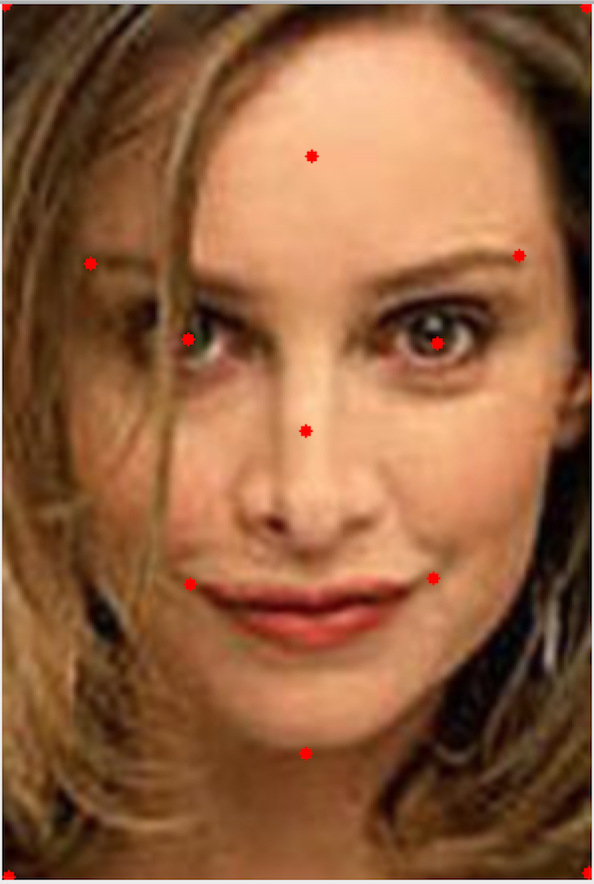
\includegraphics[width=1.0in]{beauty.png} 
  } 
  \subfigure[Lion]{ 
    %\label{fig:subfig:b} %% label for second subfigure 
    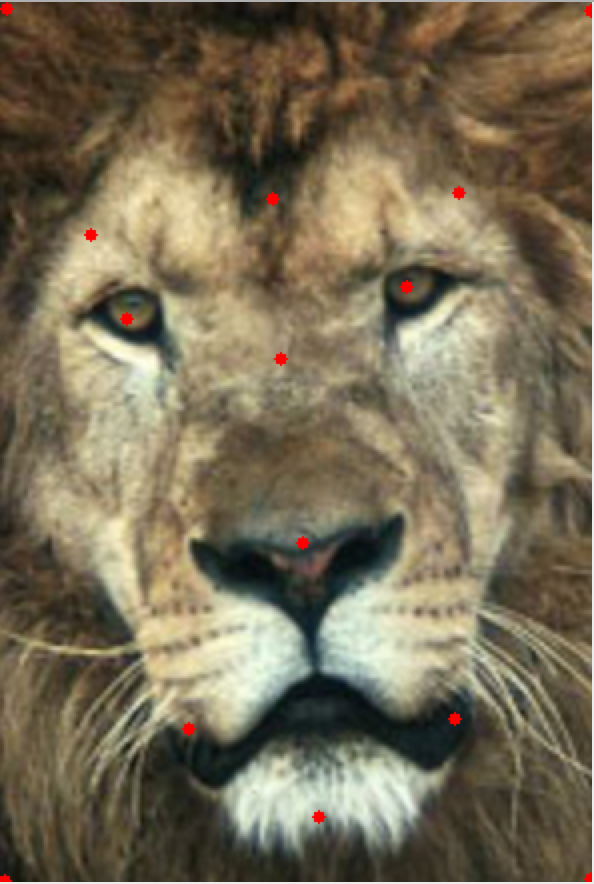
\includegraphics[width=1.0in]{lion.png} 
  } 
\end{figure}
\subsection{Delaunay三角剖分}
在这一部分,我手动实现了求Delaunay剖分的增量算法 --- Bowyer-Watson算法。算法基本思想是:从在加入新点的同时,通过更新需要改变的局部来保持一个正确的Delaunay剖分整体。步骤如下:

  \begin{figure}[htpb]
  \centering 
  \subfigure[初始化]{ 
    %\label{fig:subfig:a} %% label for first subfigure 
    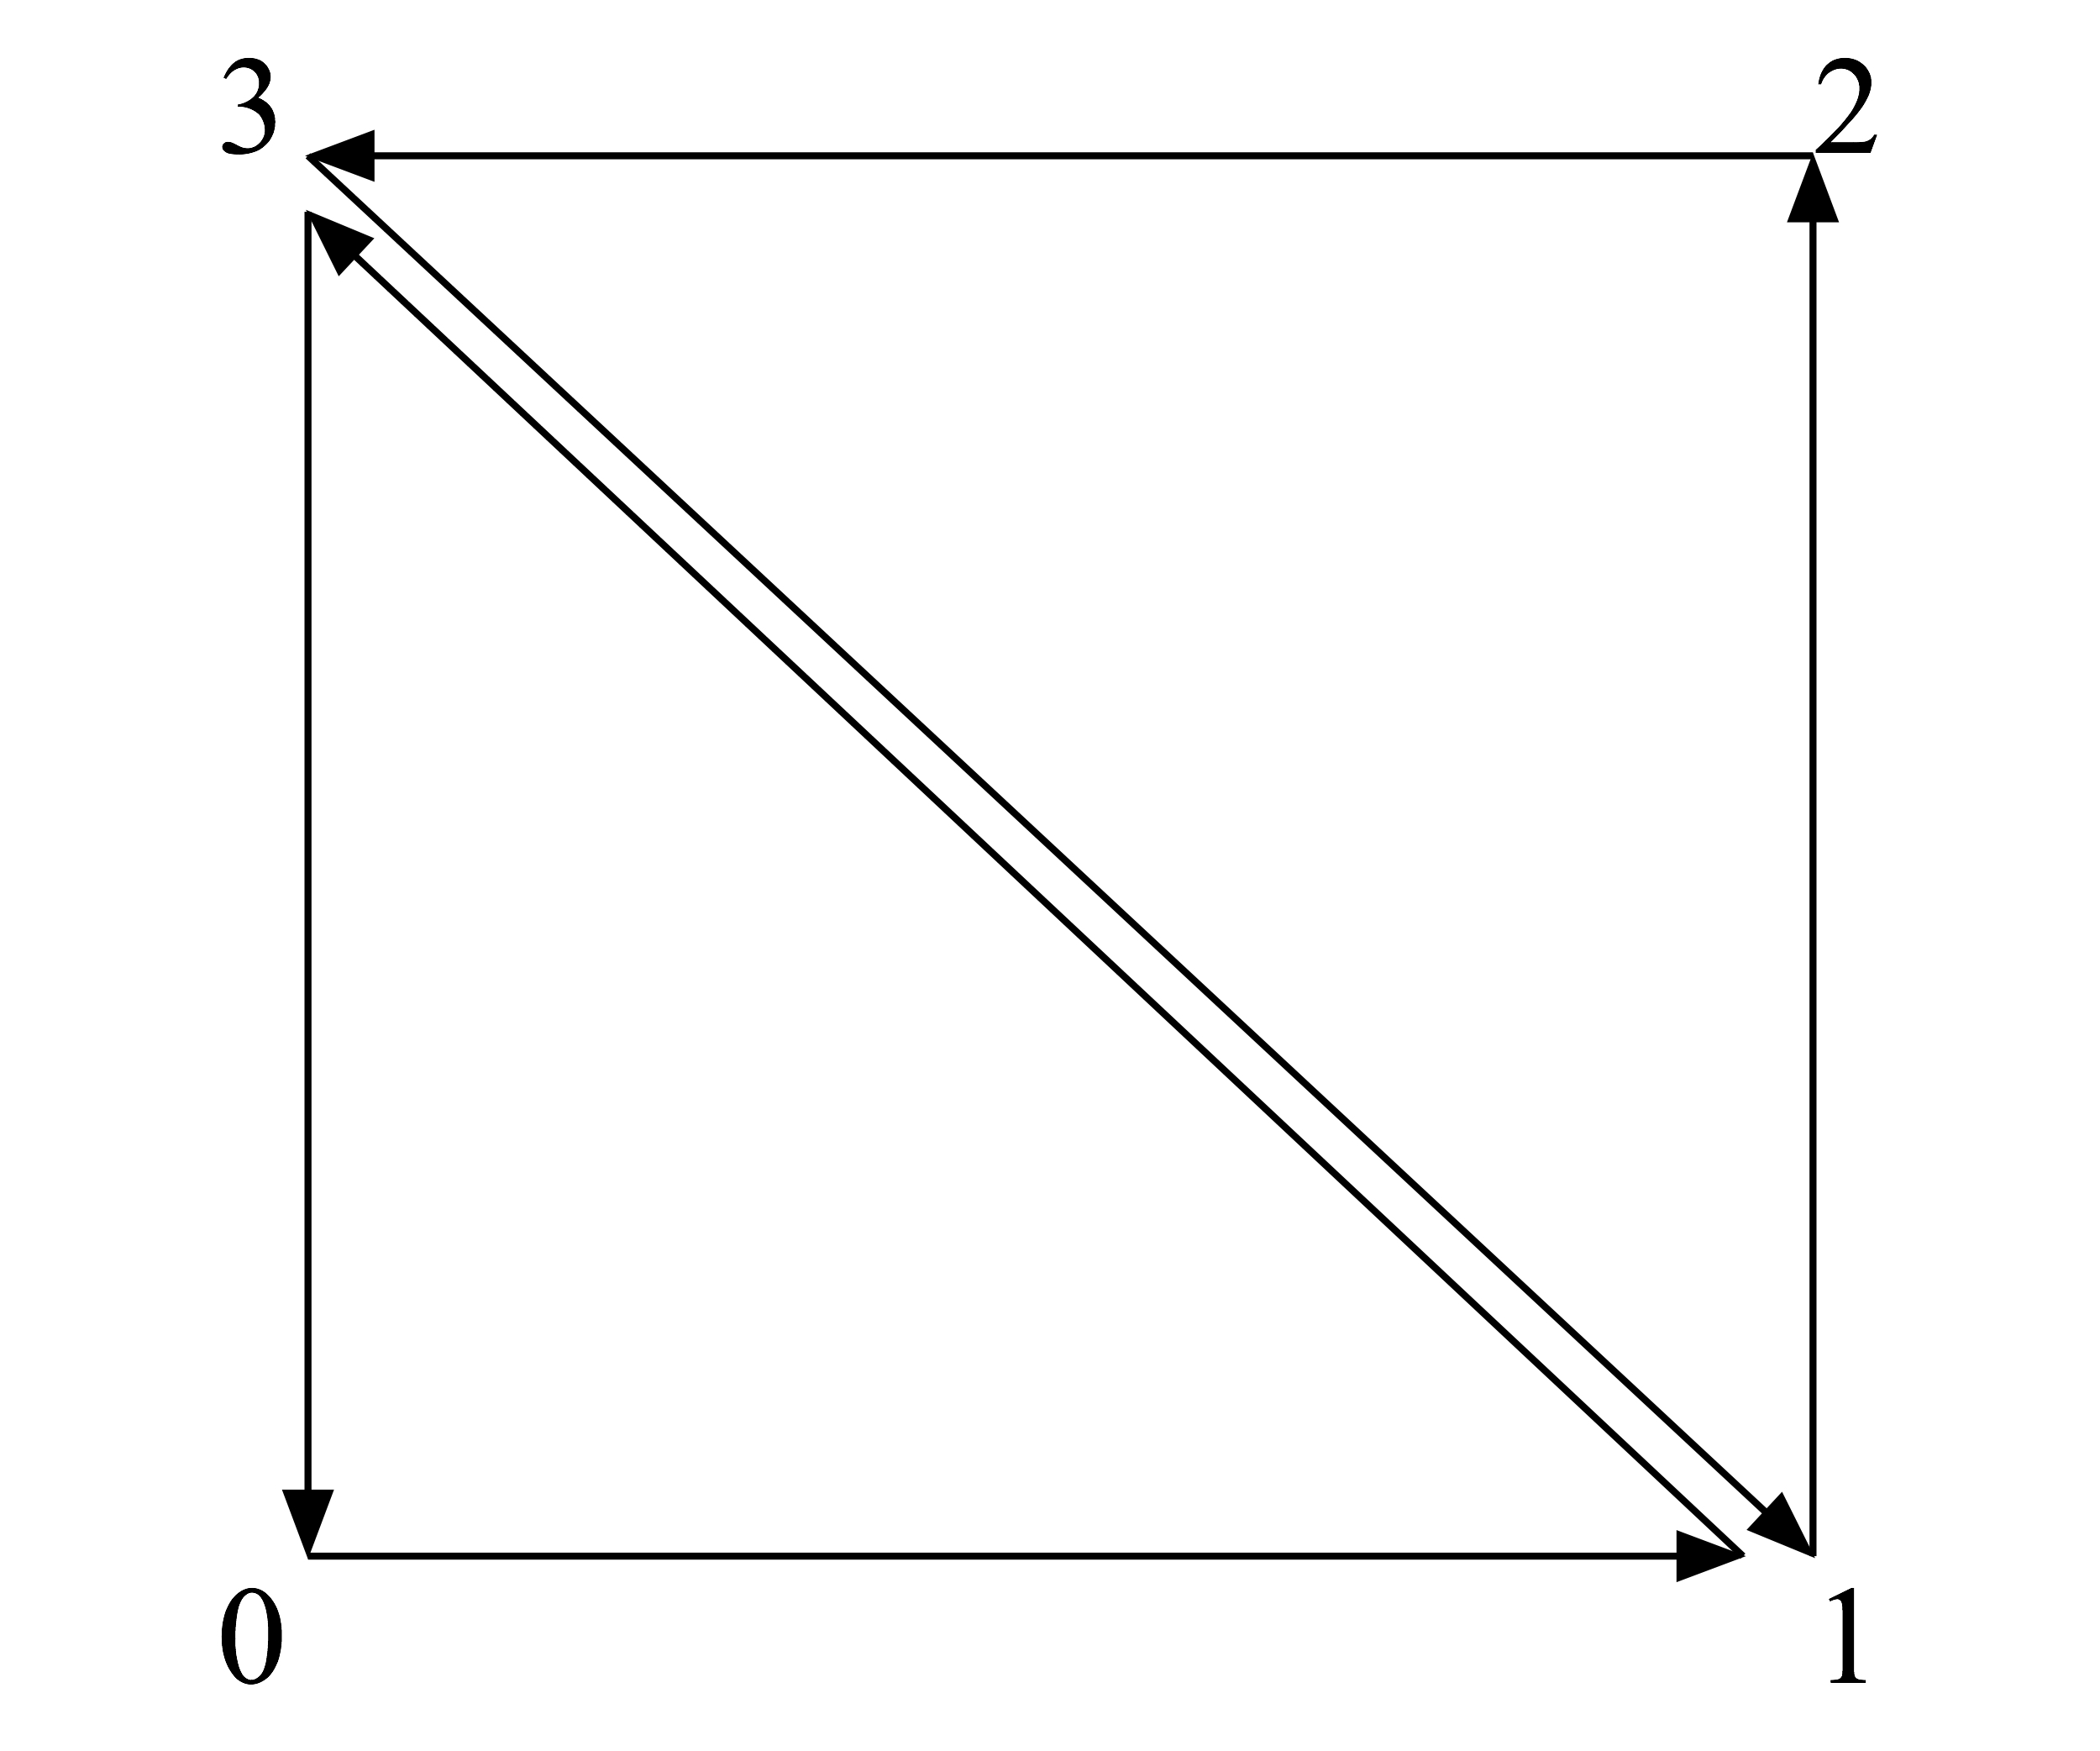
\includegraphics[width=1.0in]{fig/initial.jpg} 
  } 
  \subfigure[判断]{ 
    %\label{fig:subfig:a} %% label for first subfigure 
    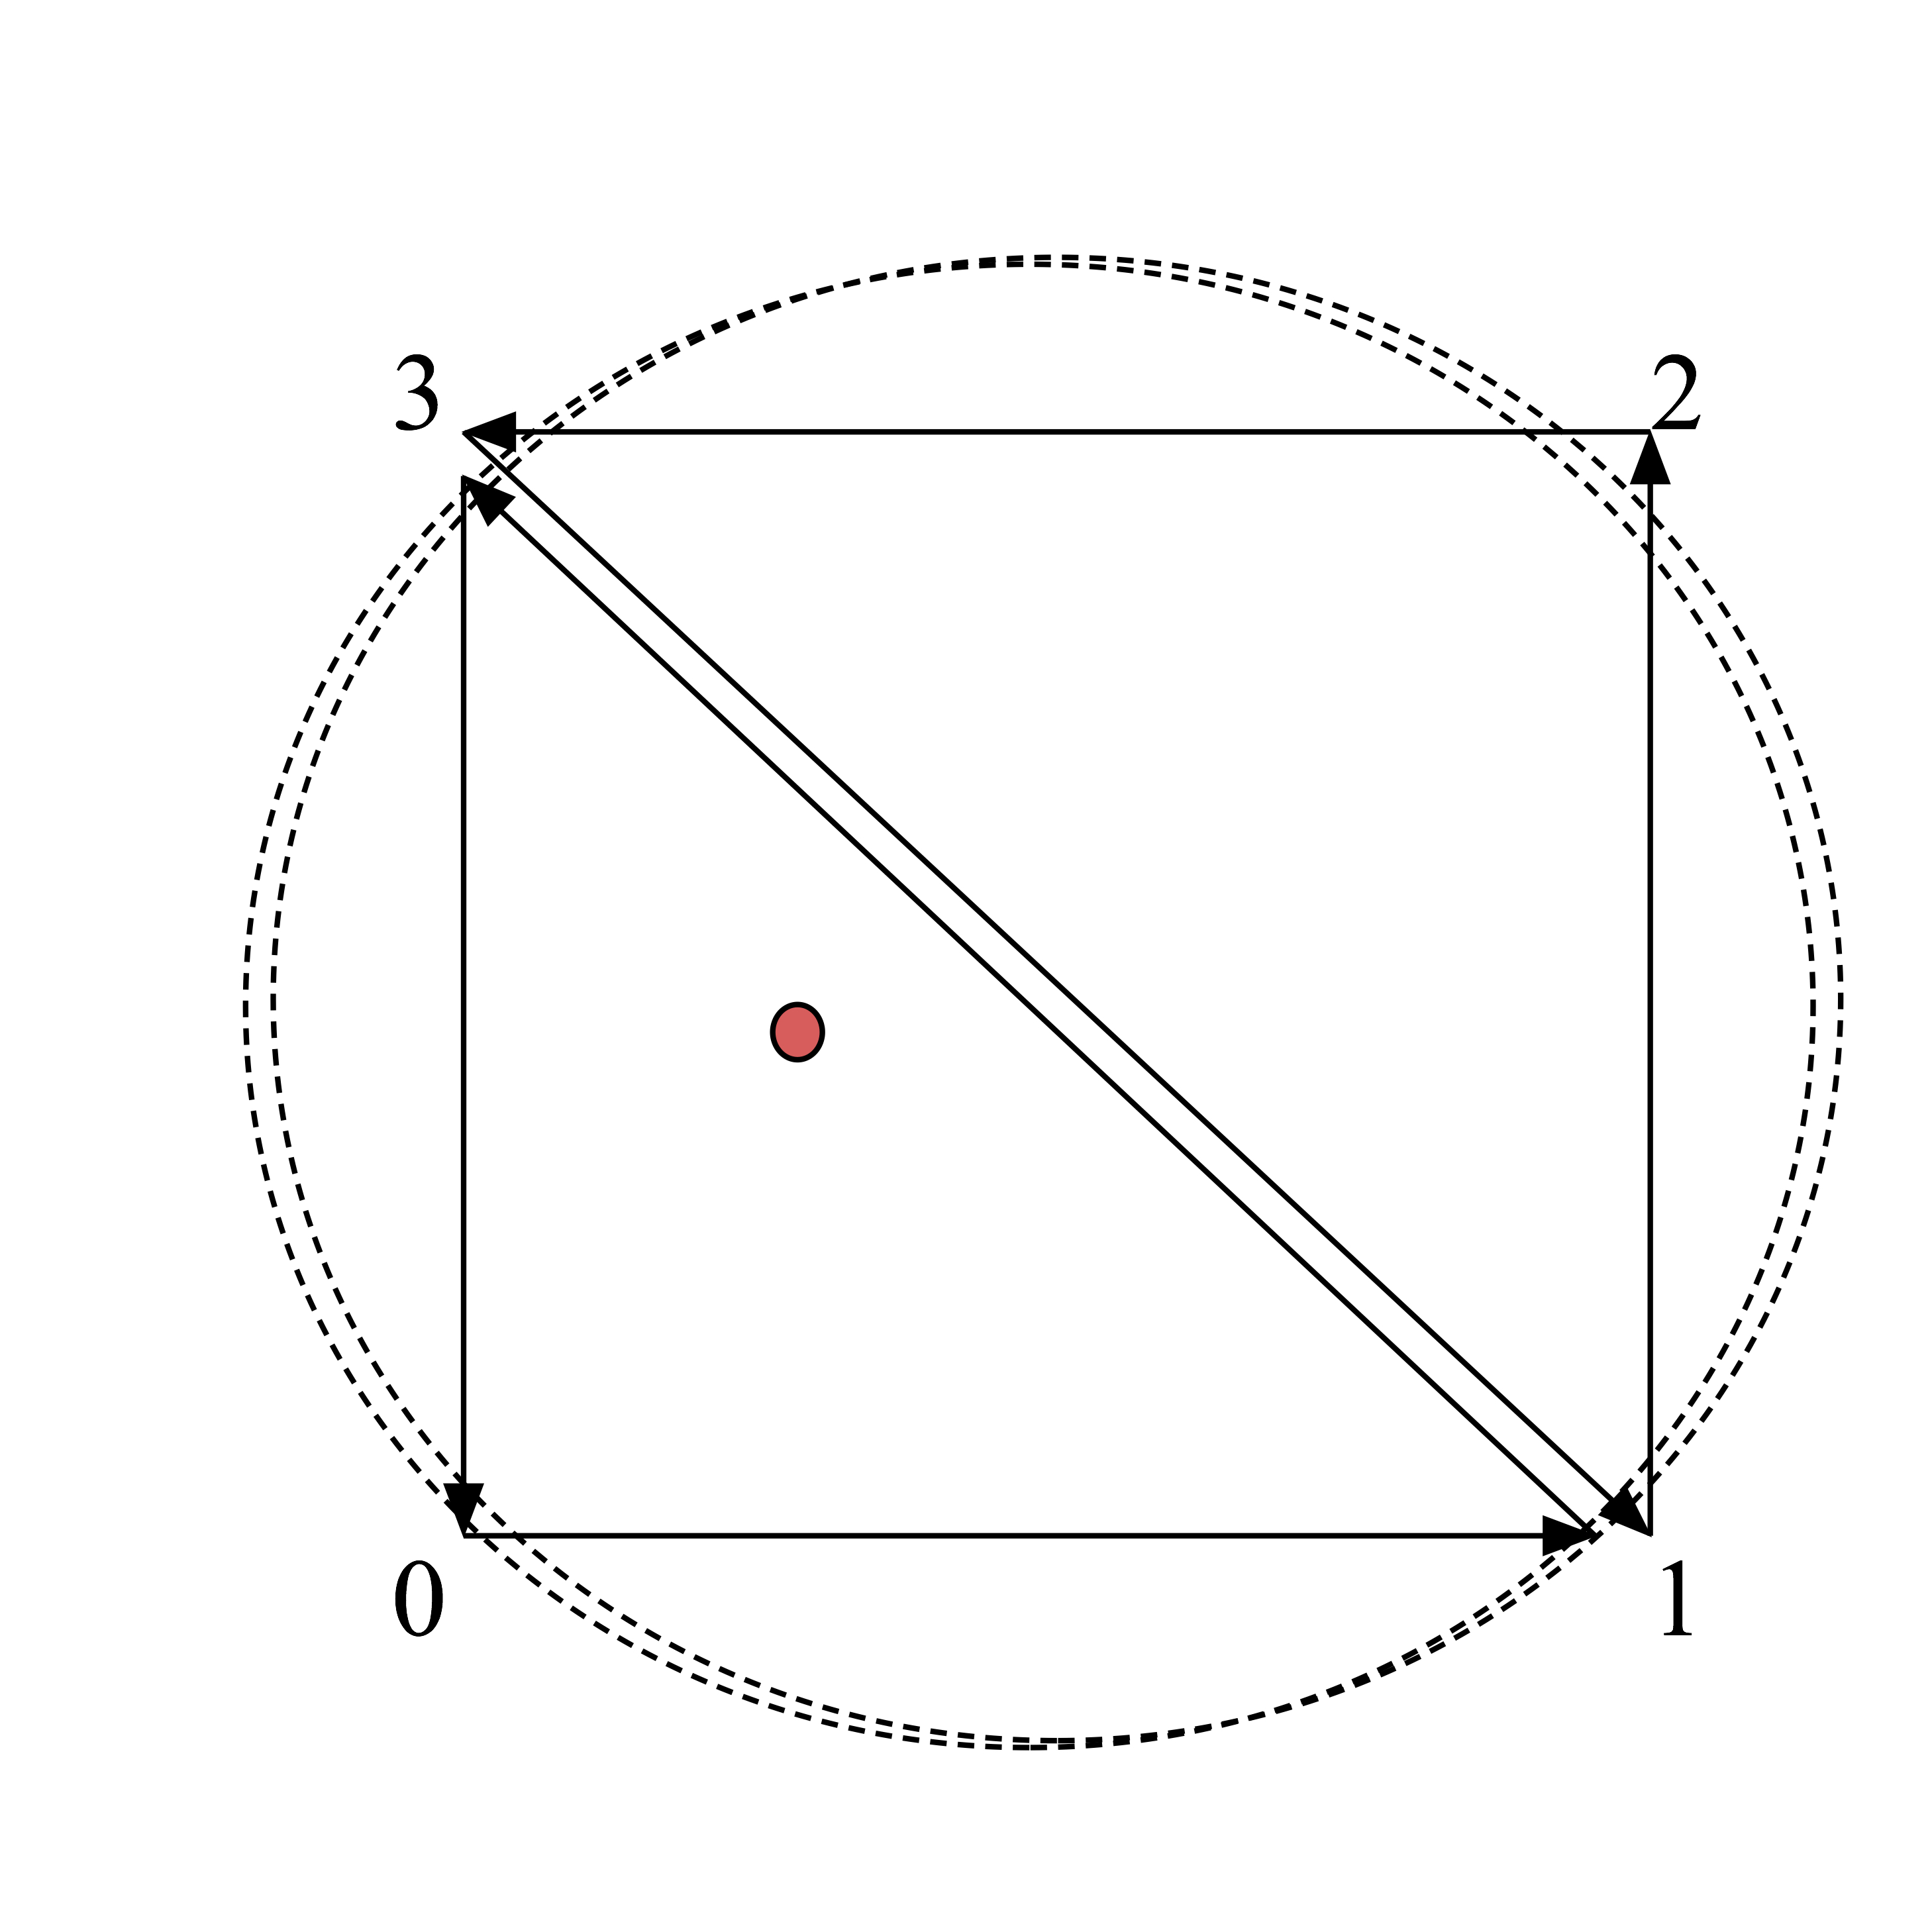
\includegraphics[width=1.0in]{fig/step1.jpg} 
  } 
  \subfigure[删除]{ 
    %\label{fig:subfig:a} %% label for first subfigure 
    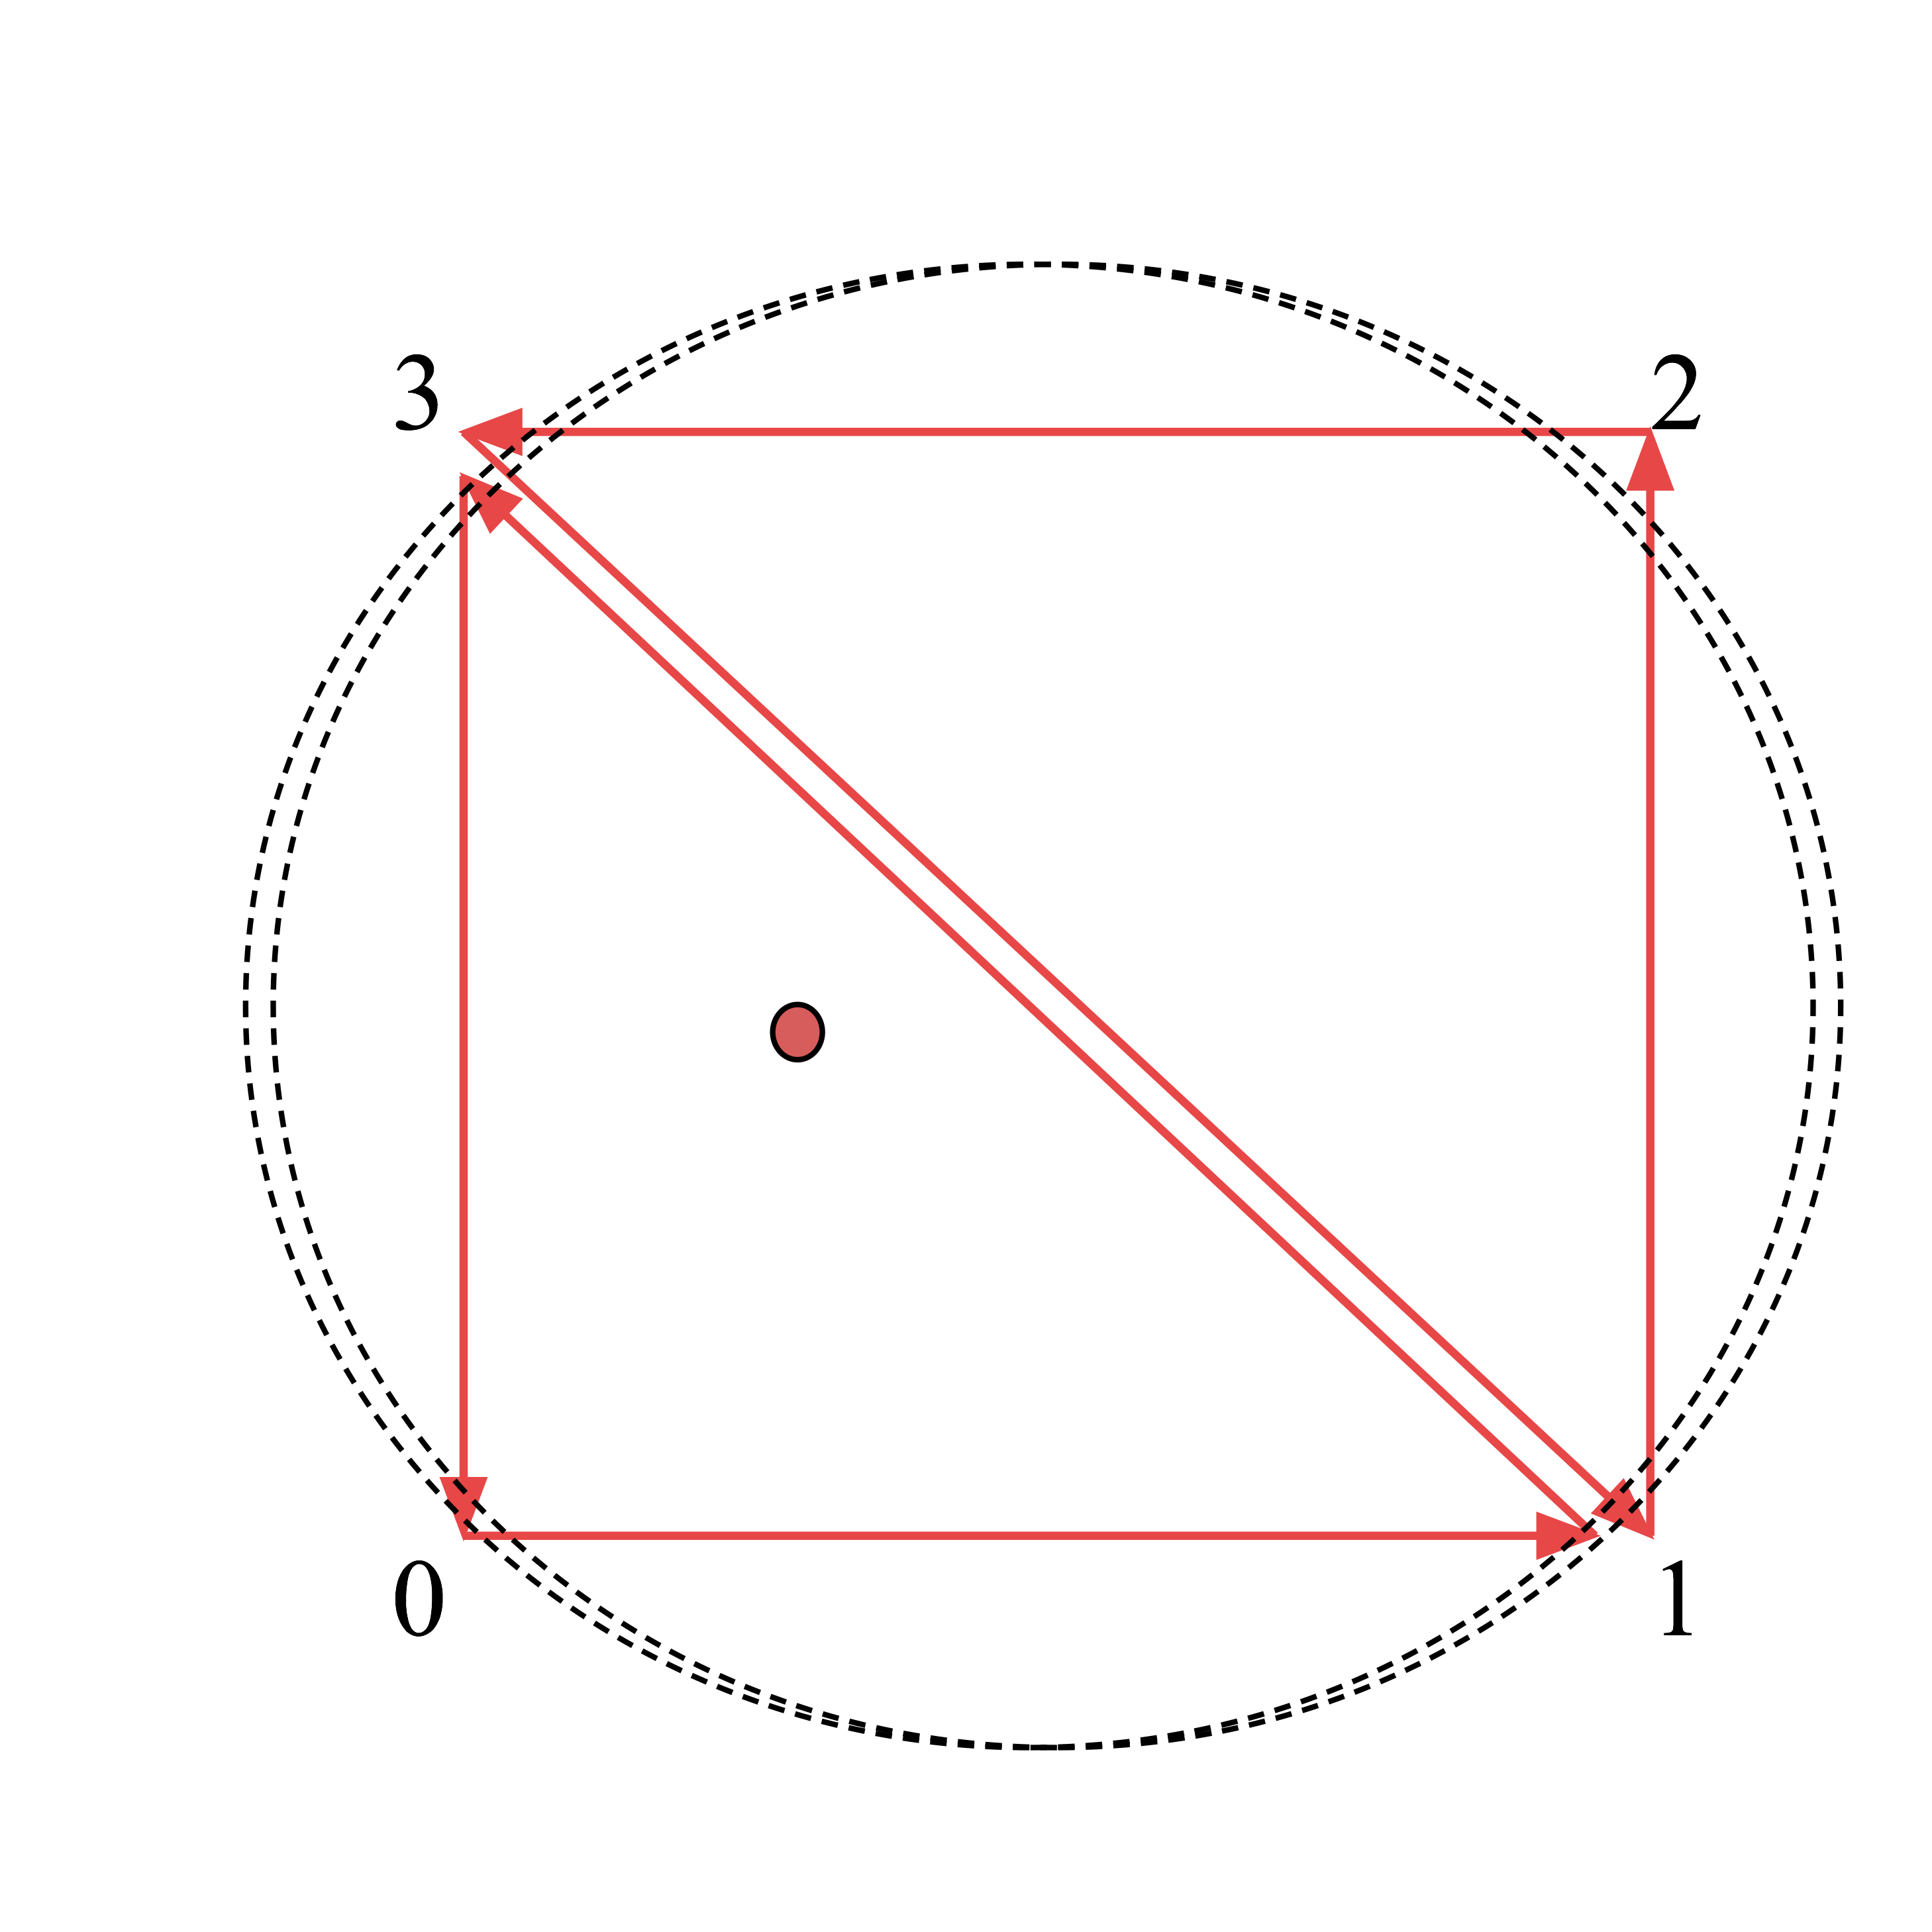
\includegraphics[width=1.0in]{fig/step2.jpg} 
  } 
  \subfigure[计算边界]{ 
    %\label{fig:subfig:a} %% label for first subfigure 
    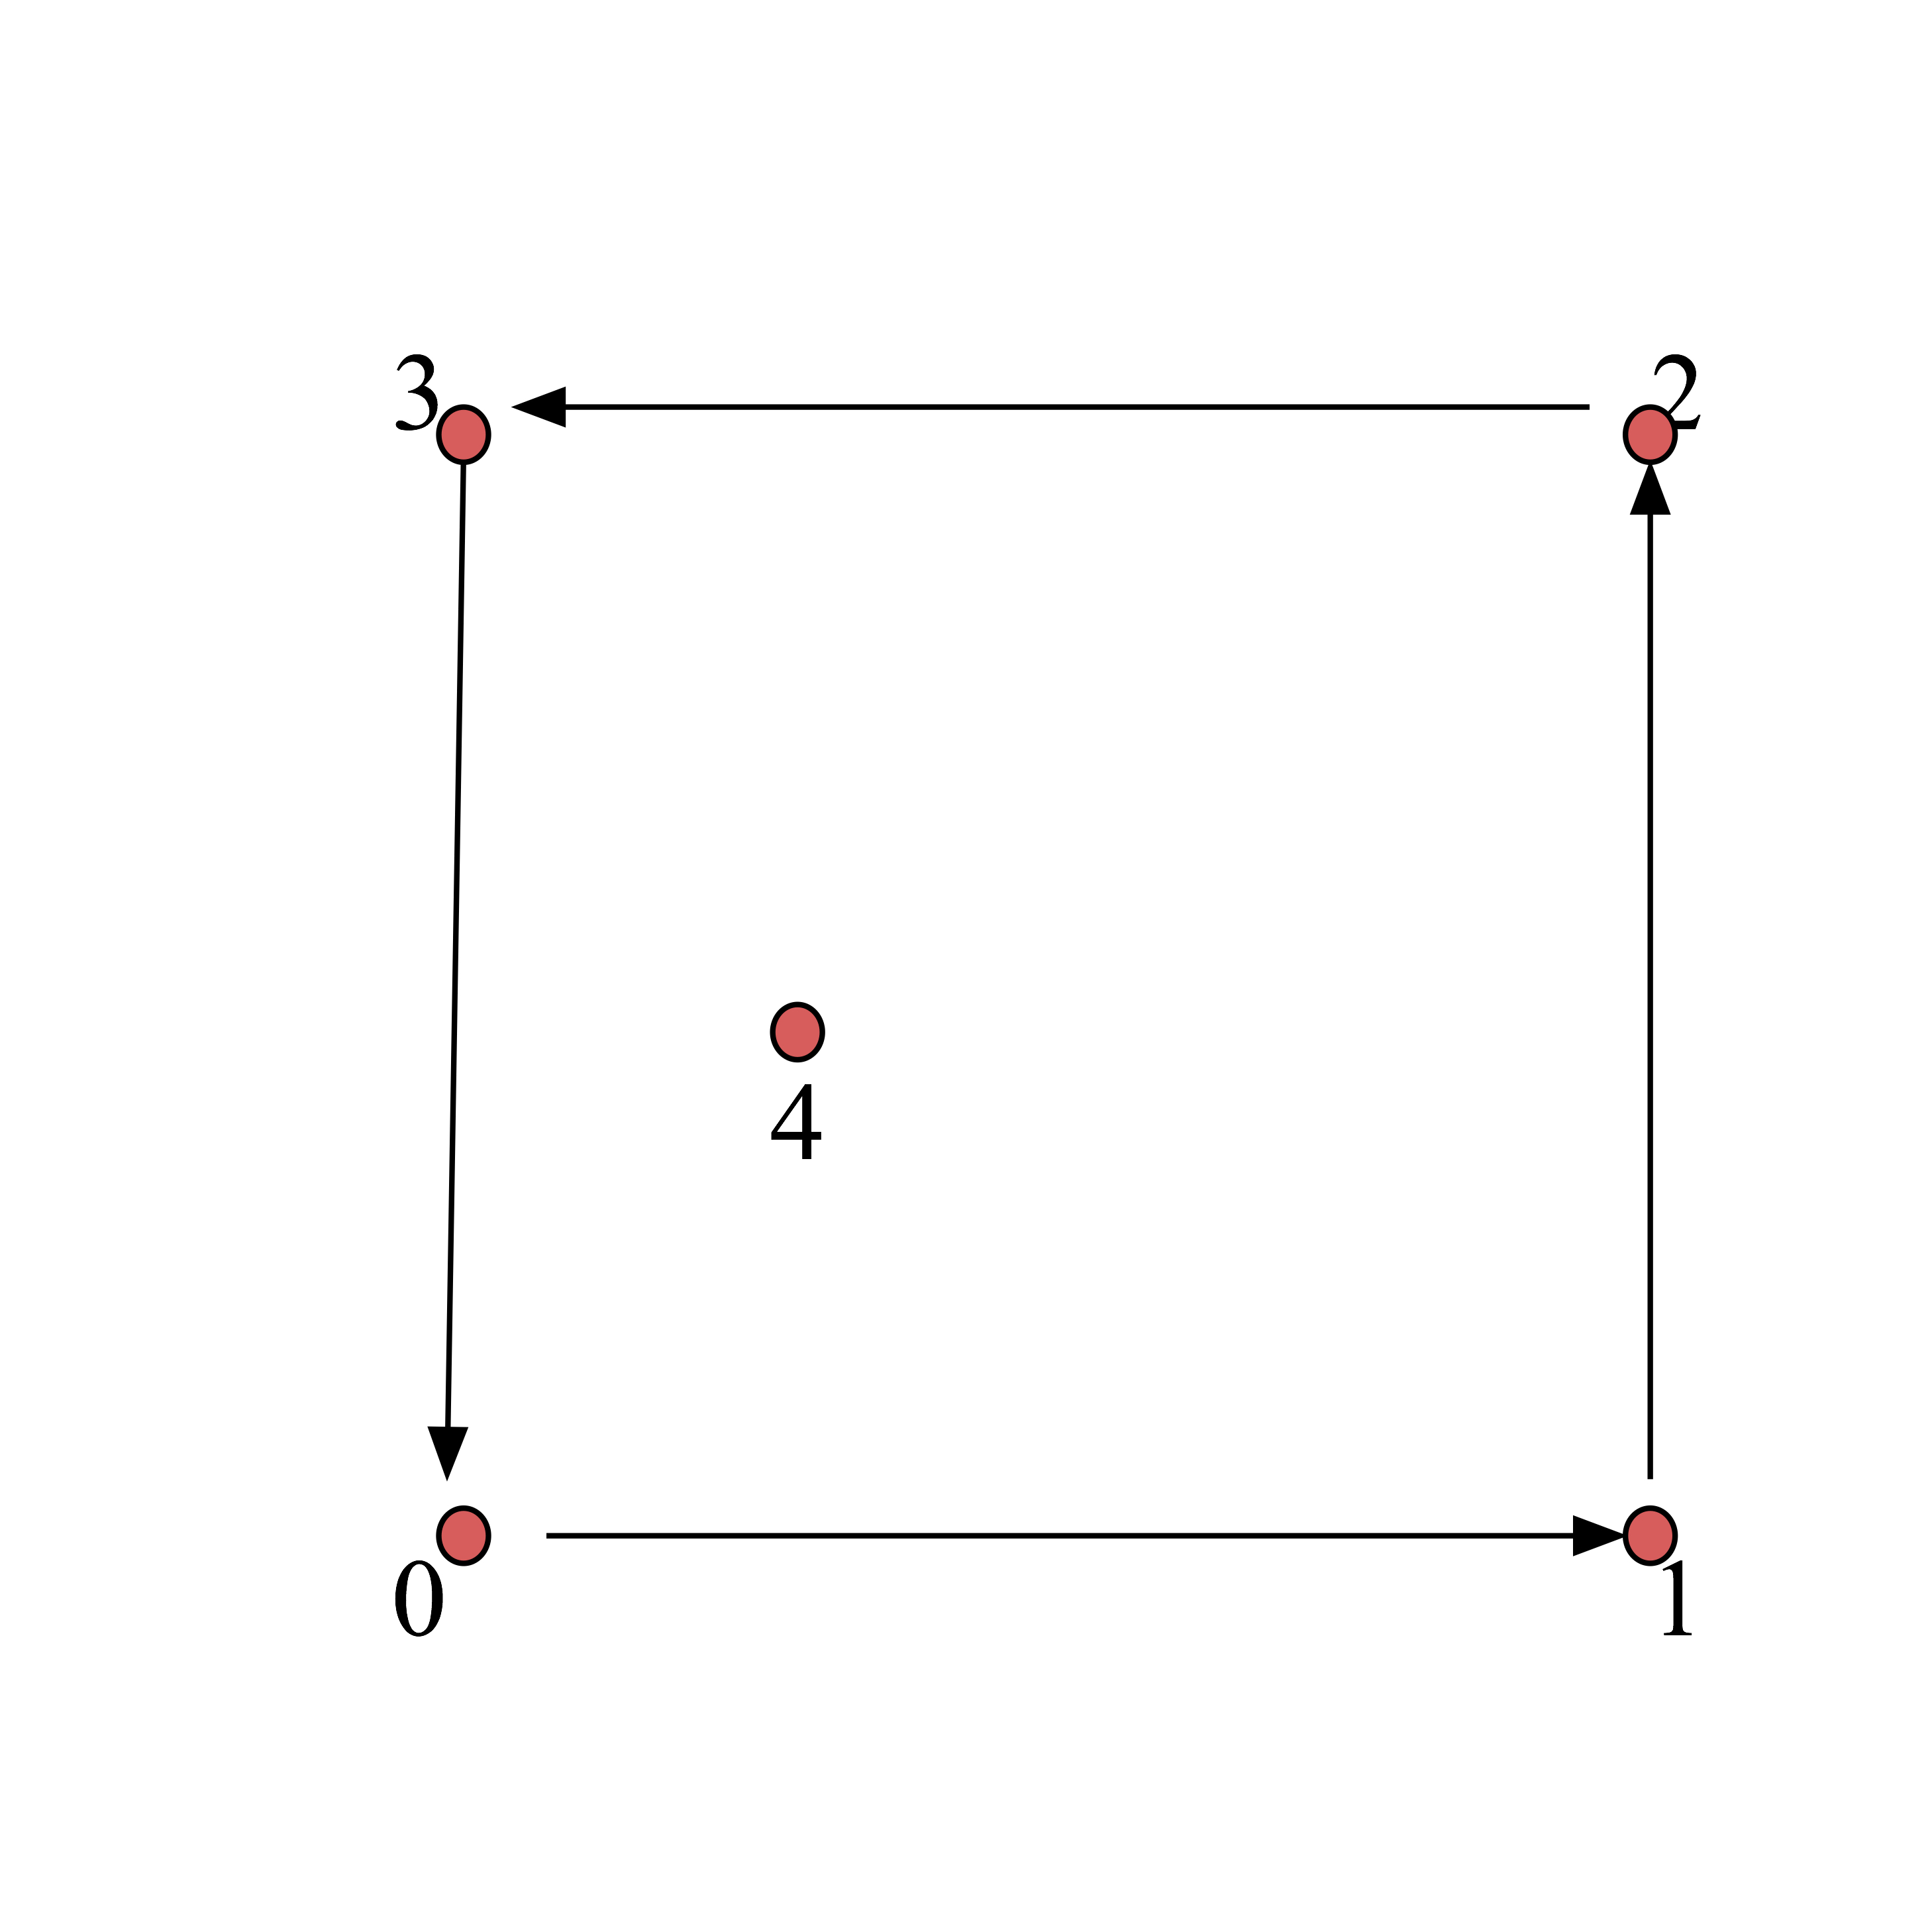
\includegraphics[width=1.0in]{fig/stepadd.jpg} 
  } 
  \subfigure[更新剖分]{ 
    %\label{fig:subfig:a} %% label for first subfigure 
    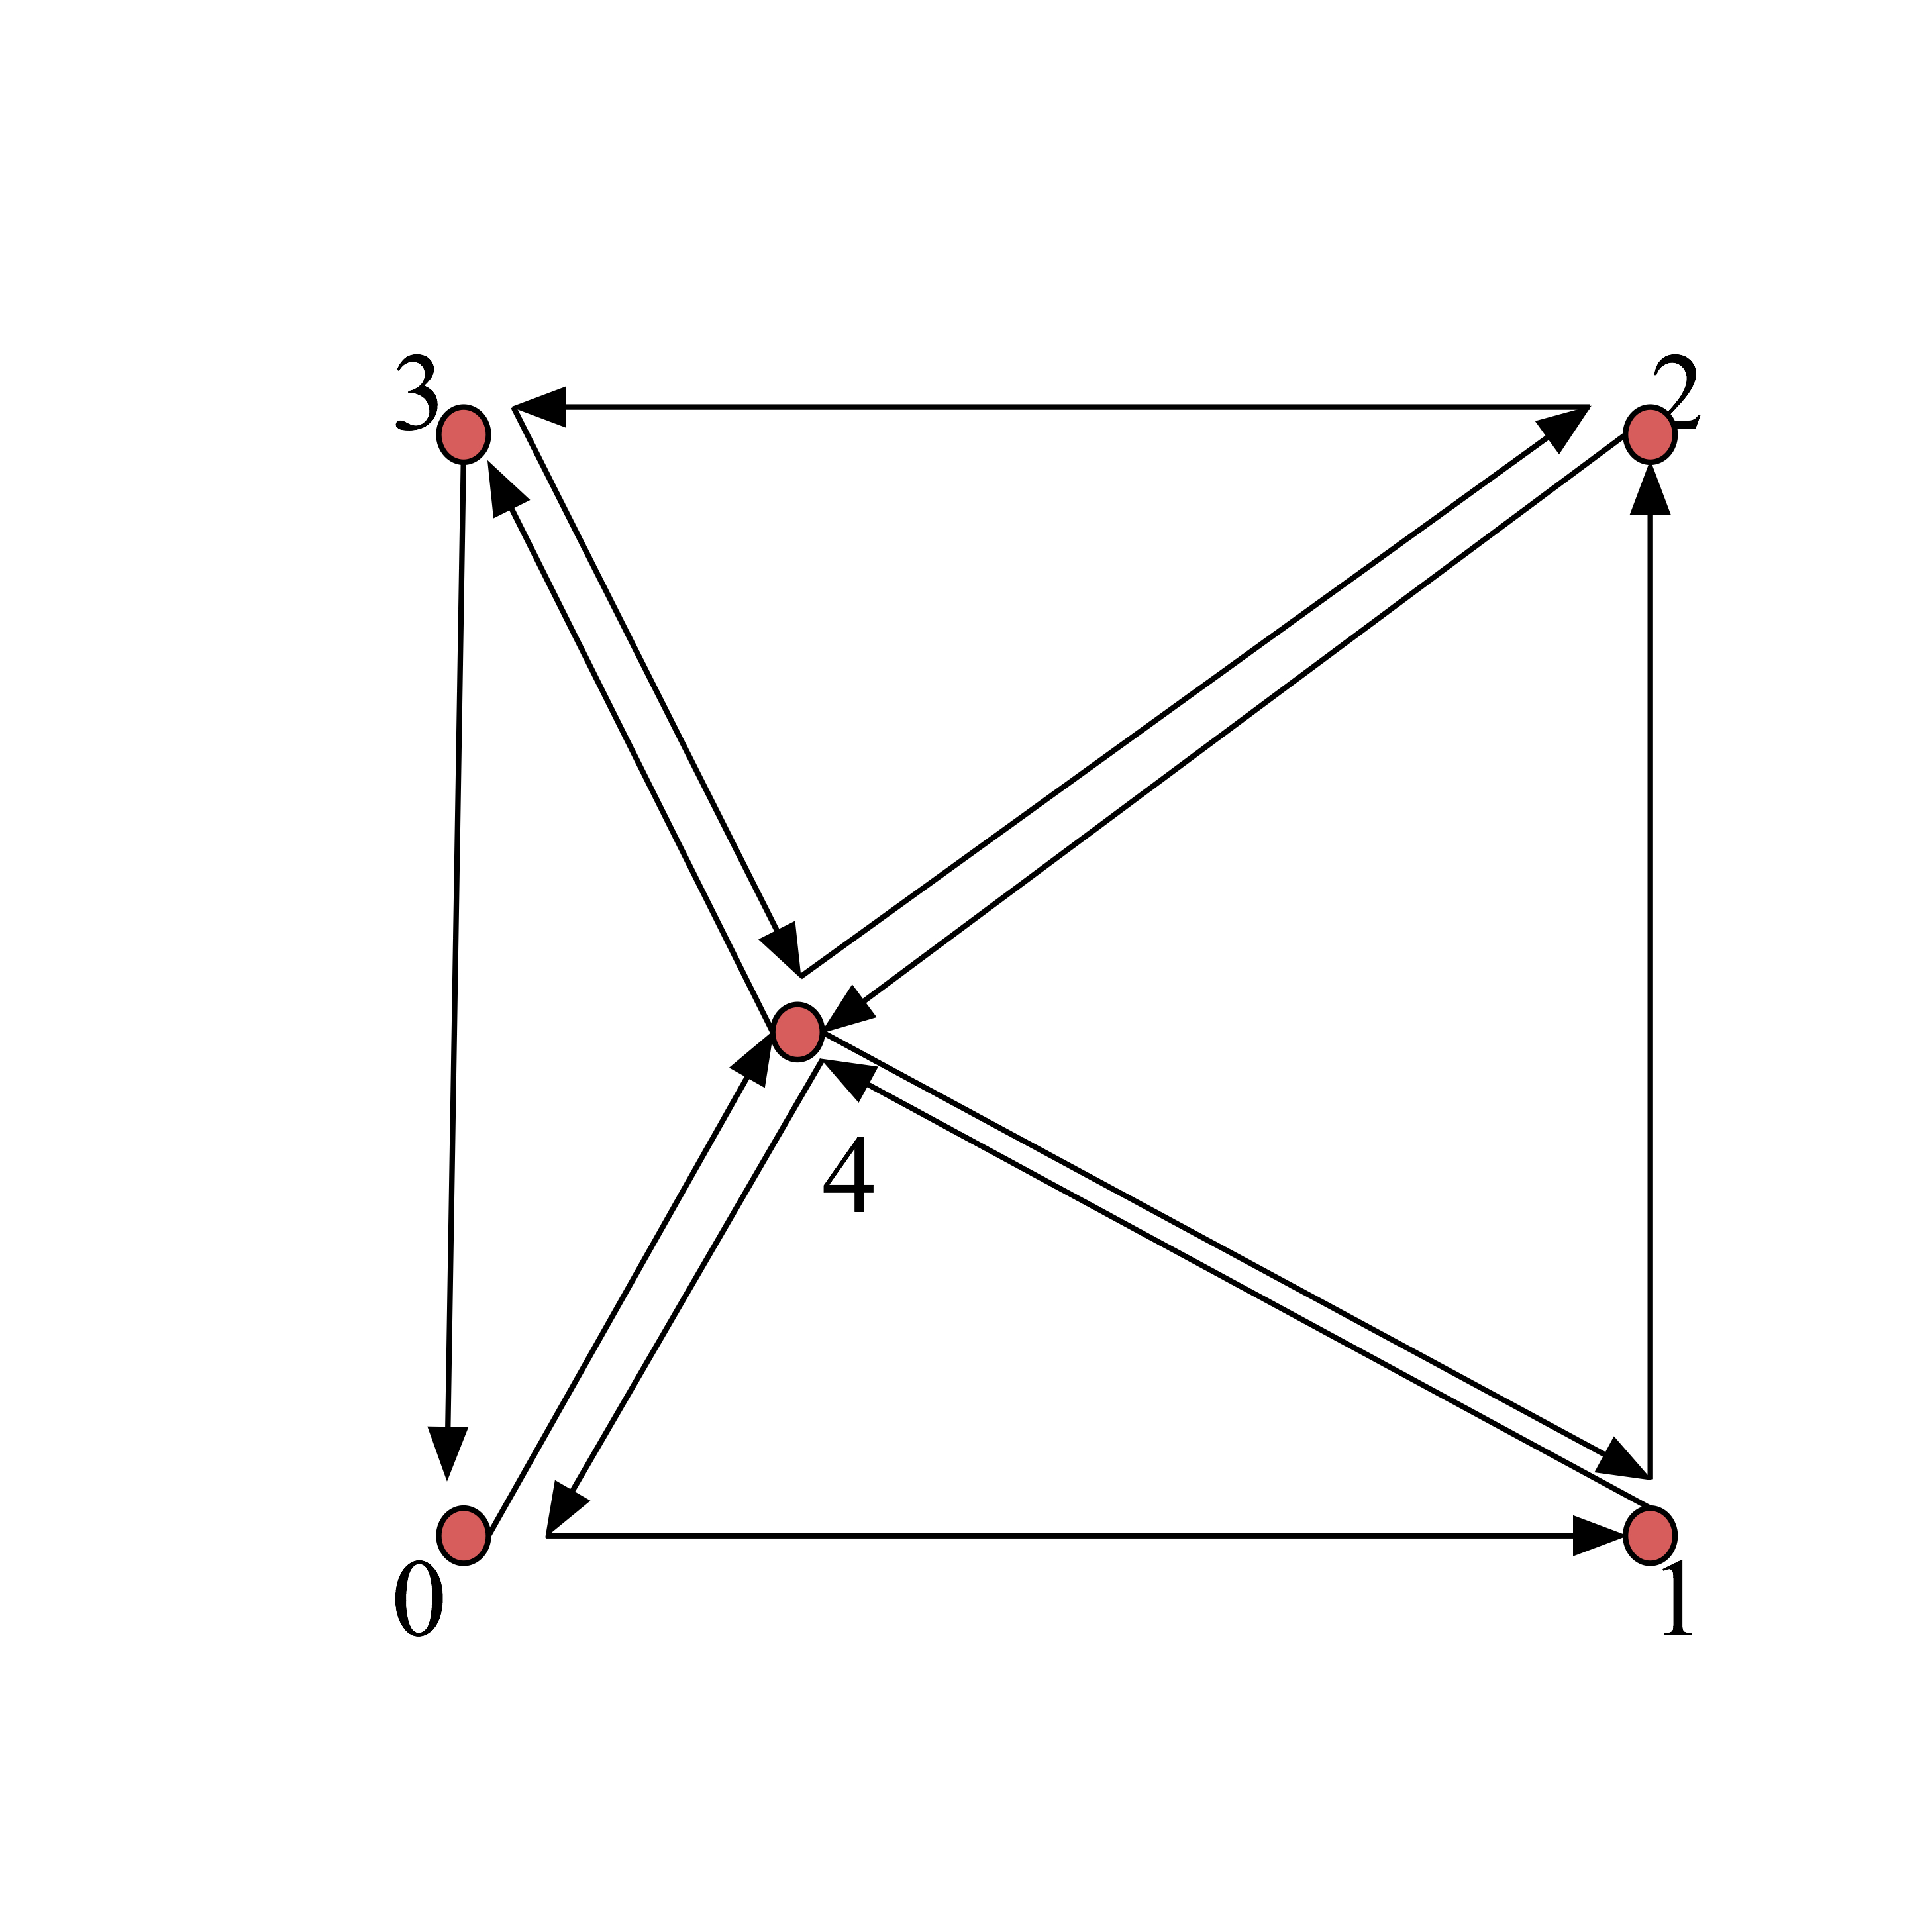
\includegraphics[width=1.0in]{fig/step3.jpg} 
  } 
\end{figure}

\begin{enumerate}
  \item 初始化;列表储存点的坐标,用dic的数据结构储存剖分,key为某个三角形对于三点的index,如$(a,b,c)$,顺序为逆时针,对应value为邻边三角形的集合,对应关系为:第$i$个邻边三角形,共享边的index为$(i+1)\%3$,$(i-1)\%3$。
  \item 判断,删除;遍历所有三角形,对每个三角形,判断其外接圆内是否含有新增点。若有,则删除剖分内该三角形。
  \item 计算边界;计算所有含有新增点的三角形集合的边界/边界点。
  \item 更新;构造新增点和边界点组成的新三角形集合(star-shaped polygon),并加入剖分中。
  \end{enumerate}
 
 核心代码如下
 \begin{lstlisting}[language=Python]
def update(tri,coor,point):  
    p = np.asarray(point)
    index = len(coor)
    coor.append(p)
    
    #check for the triangles whose circumcircle contains p
    cavity_set = []
    cavity_edge = []
    for t in tri:
        if check_circle(t,coor,p):
            cavity_set.append(t)
    T = cavity_set[0]
    e = 0
    
    while(1):  
        #T = (a,b,c), tri[T][0] is the neibor who shares edge bc
        tri_share = tri[T][e]
        p1,p2 = T[(e+1)%3], T[(e-1)%3]
        
        if tri_share in cavity_set:
            e = (tri[tri_share].index(T)+1)%3
            T = tri_share
        else:
            cavity_edge.append((p1,p2,tri_share))
            e = (e+1)%3
            if cavity_edge[0][0] == cavity_edge[-1][1]: break    
    for t in cavity_set:
        del tri[t]
        
    #star shape new triangle set
    update_tri = []
    for (p0,p1,tri_share) in cavity_edge: 
        new_tri = (index,p0,p1)
        update_tri.append(new_tri) 
        tri[new_tri] = [tri_share,None,None]
        if tri_share:
            for idx,neighbor in enumerate(tri[tri_share]):
                if neighbor:
                    if p0 in neighbor and p1 in neighbor:
                        tri[tri_share][idx] = new_tri
    update_num = len(update_tri)

    for idx, t in enumerate(update_tri):
        tri[t][1] = update_tri[(idx+1)%update_num]
        tri[t][2] = update_tri[(idx-1)%update_num]
\end{lstlisting}

\subsection{单应性矩阵变换}
\subsubsection{计算单应性矩阵}
在得到两张图片的三角剖分之后,对于一一对应的三角形组合,我们计算它的单应性矩阵,因为是仿射变换,所以这个单应性矩阵只有六个未知数。

\[
H = \begin{bmatrix}a & b & c \\ d & e & f\\0&0&1 \end{bmatrix}
\]

我们可以直接求逆得到H:
 \begin{align}
 \centering
 &HX  = X'\\
&H= X'X^{-1} = \begin{bmatrix}x'_1 & x'_2 & x'_3 \\ y'_1 & y'_2 & y'_3 \\1&1&1 \end{bmatrix}  \begin{bmatrix}x_1 & x_2 & x_3 \\ y_1 & y_2 & y_3 \\1&1&1 \end{bmatrix}^{-1}
\end{align}

\subsubsection{单应性变换}
我采用的inverse warping的方法。在变换之前,因为三角形的边界较难处理,因此我是对三角形的最小外接矩形进行warping,之后再通过masking转化回三角形。步骤如下:
\begin{enumerate}
  \item 求单应性矩阵的逆,将目标图像的点映射回原图像
\item 处理边界,对超出原图像范围的点,将其坐标投影到原图像的边界上。
\item 双线性插值所有映射点,求得他们的像素值,再映射回去得到目标图像

  \end{enumerate}
\[
I(p,q) = (1-\Delta y )(1-\Delta x) F_{00}+(1-\Delta y)\Delta x F_{10}+\Delta y(1-\Delta x)F_{01}+\Delta y \Delta x F_{11}\]
\begin{figure}[htpb]
  \centering 
  \subfigure[双线性插值]{ 
    %\label{fig:subfig:a} %% label for first subfigure 
    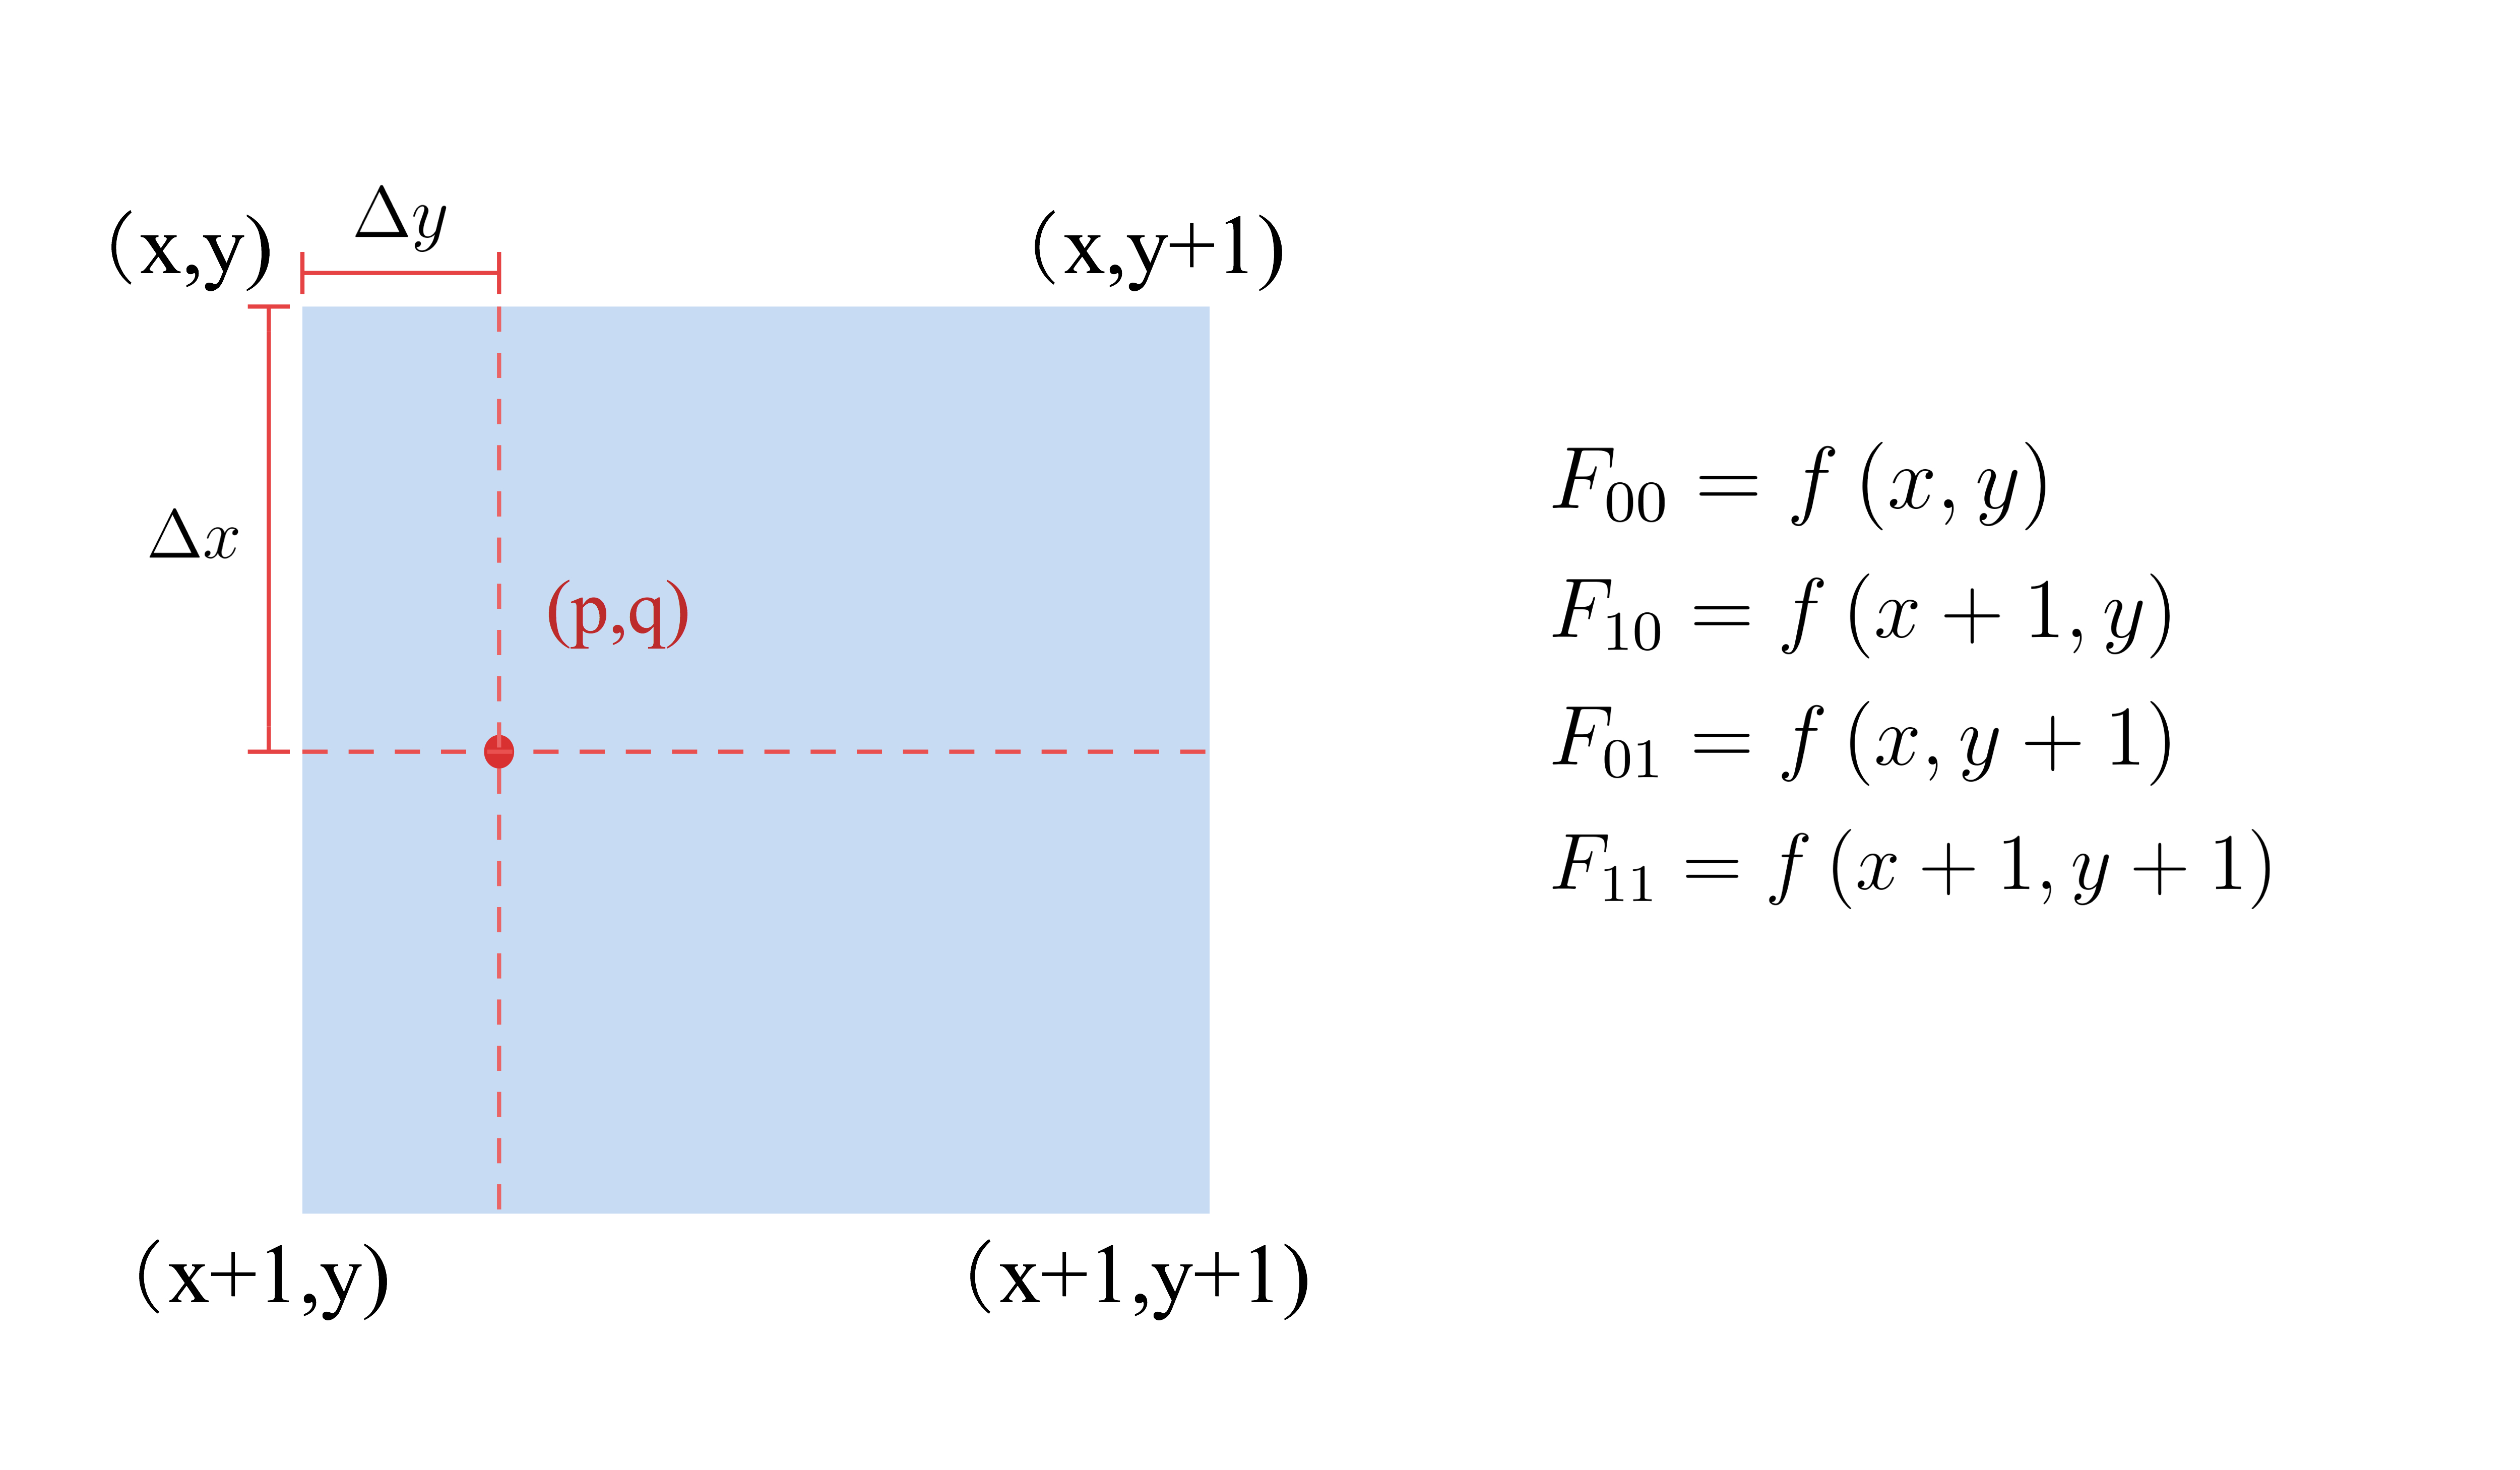
\includegraphics[width=3.0in]{fig/interpolate.jpg} 
  } 
\end{figure}
 核心代码如下
 \begin{lstlisting}[language=Python]
def apply_bilinear_interpolation(img, point):
    x = point[0]
    y = point[1] 
    if (x < 0 or y < 0
       or x > img.shape[0] - 1 or y > img.shape[1] - 1):
        if x<0:
            x = 0
        if y<0:
            y = 0
        if x > img.shape[0] - 1:
            x = img.shape[0]-1
        if y > img.shape[1] - 1:
            y = img.shape[1]-1
    delta_x =  abs(np.round(x) - x)
    delta_y =  abs(np.round(y) - y)
    x1 = int(np.round(x))
    y1 = int(np.round(y))
    I1 = img[x1][y1] * (1 - delta_x) * (1 - delta_y)
    I2 = img[int(x)][y1] * (delta_x) * (1 - delta_y)
    I3 = img[x1][int(y)] * (1 - delta_x) * (delta_y)
    I4 = img[int(x)][int(y)] * (delta_x) * (delta_y)
    return I1 + I2 + I3 + I4  #resulting intensity

def getwarped(img1Cropped,warp,r2):
    homograph = np.vstack((warp,[0,0,1]))
    inv_homo = np.linalg.inv(homograph)
    wH = r2[0]
    wW =r2[1]
    warped = np.zeros((r2[1],r2[0],3))
    for x in range(wH):
        for y in range(wW):
            pixel = np.asarray([[x],[y],[1]])
            ref_coor = np.dot(inv_homo,pixel)
            point = np.asarray([ref_coor[1][0],ref_coor[0][0]])

            intensity = [int(apply_bilinear_interpolation(img1Cropped[:,:,i], point)) for i in range(3)]

            warped[y,x,0],warped[y,x,1],warped[y,x,2] = intensity
    warped = warped.astype(np.int)  
    return warped
\end{lstlisting}
\section{效果展示}

  \begin{figure}[htpb]
  \centering 
    \subfigure[source]{ 
    %\label{fig:subfig:a} %% label for first subfigure 
    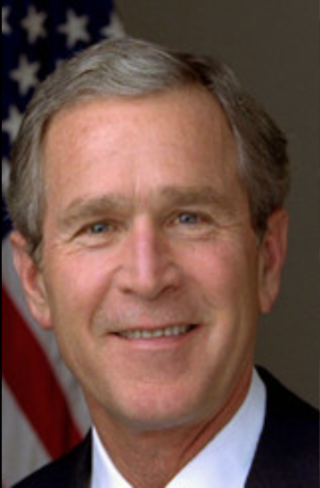
\includegraphics[width=1.0in]{fig/source1.png} 
  } 
  \subfigure[S=0.25,T=0.75]{ 
    %\label{fig:subfig:a} %% label for first subfigure 
    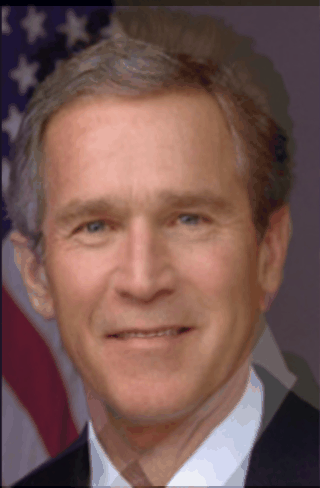
\includegraphics[width=1.0in]{fig/morph25.png} 
  } 
  \subfigure[S=0.5,T = 0.5]{ 
    %\label{fig:subfig:a} %% label for first subfigure 
    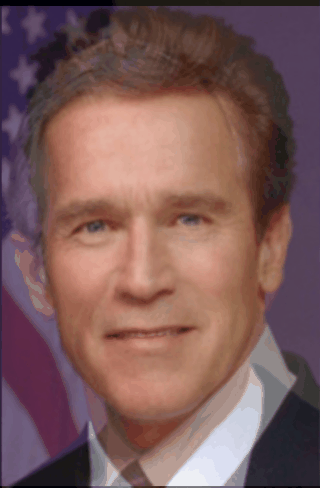
\includegraphics[width=1.0in]{fig/morph50.png} 
  } 
  \subfigure[S = 0.75,S = 0.25]{ 
    %\label{fig:subfig:a} %% label for first subfigure 
    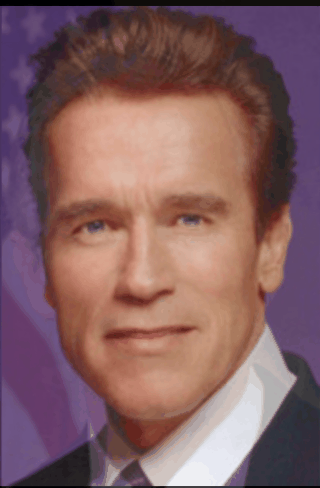
\includegraphics[width=1.0in]{fig/morph75.png} 
  } 
  \subfigure[target]{ 
    %\label{fig:subfig:a} %% label for first subfigure 
    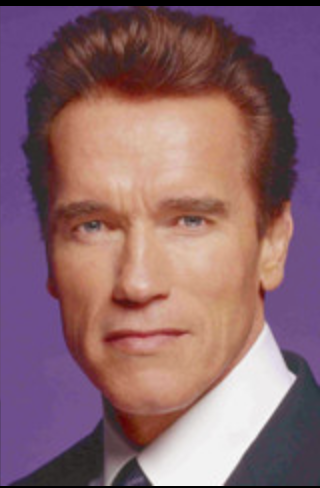
\includegraphics[width=1.0in]{fig/target1.png} 
  } 
\end{figure}



\begin{figure}[htpb]
  \centering 
  \subfigure[source]{ 
    %\label{fig:subfig:a} %% label for first subfigure 
    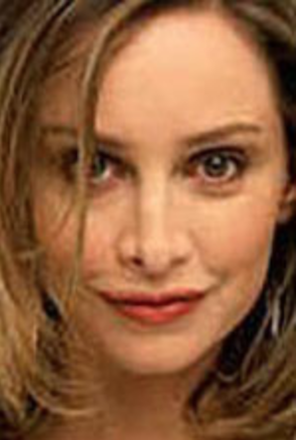
\includegraphics[width=1.0in]{fig/source2.png} 
  } 
  \subfigure[S=0.25,T=0.75]{ 
    %\label{fig:subfig:a} %% label for first subfigure 
    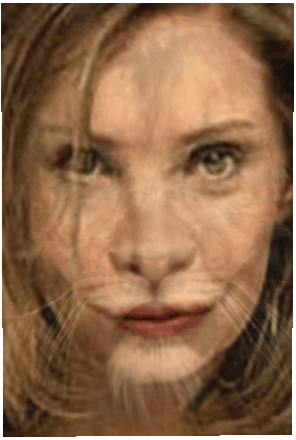
\includegraphics[width=1.0in]{fig/morph75-2.png} 
  } 
  \subfigure[S=0.5,T = 0.5]{ 
    %\label{fig:subfig:a} %% label for first subfigure 
    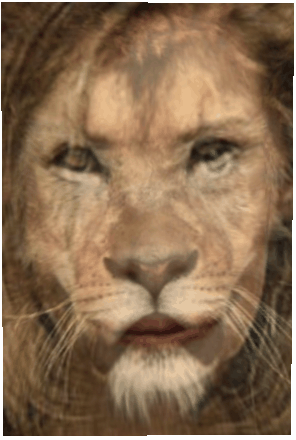
\includegraphics[width=1.0in]{fig/morph50-2.png} 
  } 
  \subfigure[S = 0.75,S = 0.25]{ 
    %\label{fig:subfig:a} %% label for first subfigure 
    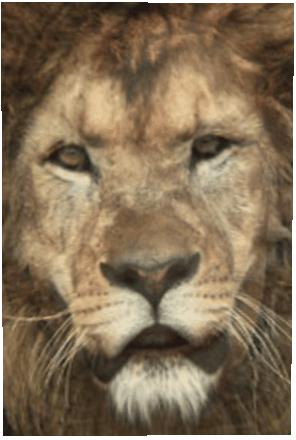
\includegraphics[width=1.0in]{fig/morph25-2.png} 
  } 
    \subfigure[target]{ 
    %\label{fig:subfig:a} %% label for first subfigure 
    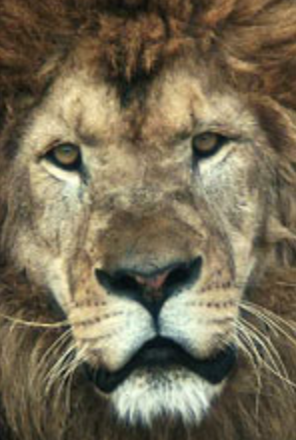
\includegraphics[width=1.0in]{fig/target2.png} 
  } 

\end{figure}

\end{document}
